\documentclass[12pt,a4paper]{article}
\usepackage{amsmath}
\usepackage{amssymb}
\usepackage{graphicx}
\usepackage{hyperref}
\usepackage{natbib}
\usepackage{url}
\usepackage{xcolor}
\usepackage{booktabs}
\usepackage{caption}
\usepackage{subcaption}
\usepackage{setspace}
\usepackage{geometry}
\usepackage{float}
\usepackage{enumitem}
\usepackage{fancyhdr}
\usepackage{microtype}
\usepackage[T1]{fontenc}
\usepackage{lmodern}
\usepackage{pdflscape}

% Set headheight to fix fancyhdr warning
\setlength{\headheight}{14.5pt}

% Set page geometry
\geometry{
 a4paper,
 total={170mm,257mm},
 left=20mm,
 right=20mm,
 top=20mm,
 bottom=20mm,
}

% Configure section heading formatting
\usepackage{titlesec}
\titleformat{\section}{\large\bfseries}{\thesection}{1em}{}
\titleformat{\subsection}{\normalsize\bfseries}{\thesubsection}{1em}{}

% Configure fancy headers
\pagestyle{fancy}
\fancyhf{}
\fancyhead[L]{Enhancing Nitrate Removal in Denitrifying Woodchip Bioreactors}
\fancyhead[R]{\thepage}
\renewcommand{\headrulewidth}{0.4pt}

% Configure hyperref
\hypersetup{
    colorlinks=true,
    linkcolor=blue,
    filecolor=magenta,
    urlcolor=blue,
    citecolor=blue,
    pdftitle={Enhancing Nitrate Removal in Denitrifying Woodchip Bioreactors},
    pdfauthor={Reza Moghaddam and Laura E. Christianson},
}

% Configure figure and table placement
\renewcommand{\topfraction}{0.85}
\renewcommand{\bottomfraction}{0.85}
\renewcommand{\textfraction}{0.1}
\renewcommand{\floatpagefraction}{0.75}

\title{Enhancing Nitrate Removal in Denitrifying Woodchip Bioreactors: A Comprehensive Analysis of Enhancement Strategies and Environmental Trade-offs}
\author{Reza Moghaddam\textsuperscript{1,*} and Laura E. Christianson\textsuperscript{2}}
\date{\today}

\begin{document}

\maketitle

\begin{center}
\footnotesize
\textsuperscript{1}Earth Sciences New Zealand\\
\textsuperscript{2}Research Associate Professor, Department of Crop Sciences, University of Illinois at Urbana-Champaign\\
S-322 Turner Hall, Urbana, IL 61801, USA\\
*Corresponding author: reza.moghaddam@niwa.co.nz
\end{center}

\begin{abstract}
Denitrifying woodchip bioreactors function as passive treatment systems that utilize naturally occurring bacteria to remove nitrate from agricultural drainage water and other contaminated sources. However, their performance can be limited by factors such as temperature, carbon availability, and hydraulic conditions. This systematic review synthesizes current knowledge on enhancement strategies for woodchip bioreactors to optimize nitrate removal while minimizing unintended environmental consequences. We systematically reviewed 70 peer-reviewed studies examining various enhancement approaches, including carbon supplementation, alternative media (carbon sources other than standard woodchips, such as corn cobs, agricultural residues, and different wood species), bioaugmentation, hydraulic optimization, mixed media systems, and hybrid systems. Our analysis indicates that carbon dosing and alternative media can achieve the highest nitrate removal rates (up to 38 g N/m$^3$/day), but may introduce additional operational complexity and costs. Temperature sensitivity varies significantly among enhancement strategies, with Q$_{10}$ values ranging from 1.8 to 3.0, with aged woodchips showing higher temperature dependence than fresh materials. Additionally, we address the potential for pollution swapping, particularly regarding dissolved organic carbon leaching, phosphorus dynamics, and greenhouse gas emissions. This integrated analysis provides guidance for selecting enhancement strategies based on site-specific conditions, regulatory requirements, and operational constraints.
\end{abstract}

\section{Introduction}

Elevated nitrate concentrations in water bodies contribute to eutrophication, harmful algal blooms, hypoxic zones, and can pose risks to human health when present in drinking water sources \citep{RN1181}. Nitrate pollution originates from multiple sources including agricultural subsurface drainage, aquaculture and other wastewaters, septic effluent, point sources, and urban runoff \citep{RN1181, RN310}. As agricultural production has intensified to meet global food demands and urbanization has expanded, the challenge of managing nitrate pollution has become increasingly urgent \citep{RN312}.

Various nitrate removal technologies have been developed and implemented to address this water quality challenge \citep{RN625, RN826}. Physical-chemical methods include ion exchange, reverse osmosis, and electrochemical processes, which can achieve high removal efficiencies (>90\%) but typically require high energy inputs and generate concentrated waste streams \citep{RN625}. Constructed wetlands provide effective treatment with lower operational costs but require substantial land areas and may have variable performance under different climatic conditions \citep{RN826}. Biological treatment systems, including activated sludge processes and membrane bioreactors, offer reliable performance but involve higher capital and operational costs \citep{RN625}. In-field management practices such as precision nutrient management, cover crops, and controlled drainage systems aim to reduce nitrate at the source but may provide incomplete protection during high-loading events \citep{RN826}.

Denitrifying woodchip bioreactors represent a practical and relatively low-cost edge-of-field treatment system designed to remove nitrate from various water sources \citep{RN625, RN310}. These systems utilize a carbon-rich woodchip medium to support microbial denitrification, a process where nitrate is reduced to nitrogen gas (N$_{2}$) under anoxic conditions \citep{RN242, RN629}. Since their introduction, woodchip bioreactors have demonstrated potential for nitrate removal in treating subsurface drainage, surface runoff, aquaculture effluent, and other point sources. Field-scale systems typically achieve nitrate removal rates ranging from 0.01 to 22 g N/m$^3$/day, with lower rates often associated with nitrate limitations \citep{RN625, RN310}.

Compared to other treatment technologies, woodchip bioreactors offer several advantages including minimal energy requirements and the ability to operate under variable flow conditions (typically ranging from 0.1 to 10 times the design flow rate) \citep{RN625, RN310}. Long-term studies indicate that these systems can maintain nitrate removal for up to 15 years without further maintenance or carbon supplementation because wood chips degrade sufficiently slowly under anoxic conditions \citep{RN625, RN629}.

However, conventional woodchip bioreactors face several limitations that constrain their widespread implementation and effectiveness. Performance is often limited by carbon availability, particularly under cold conditions or high nitrate loading \citep{RN625, RN228, RN258}. Temperature effects can reduce removal rates significantly in winter months, while hydraulic short-circuiting and variable flow conditions can compromise treatment efficiency in field settings \citep{RN228, RN309}. Additionally, space constraints, cost considerations, and the need for higher removal rates to meet water quality targets have motivated research into enhancement strategies.

\textbf{Research Objectives and Questions}

This systematic review addresses the growing body of research on woodchip bioreactor enhancement strategies. Specifically, we address the following research questions:

1. \textit{How effective are different enhancement strategies in improving nitrate removal rates and efficiency compared to conventional woodchip bioreactors?}

2. \textit{How do environmental factors such as temperature, hydraulic retention time, and influent nitrate concentration affect the performance of enhanced bioreactors?}

3. \textit{What are the environmental trade-offs associated with enhancement strategies, including impacts on greenhouse gas emissions, dissolved organic carbon leaching, and phosphorus dynamics?}

4. \textit{What are the economic implications and practical considerations for implementing different enhancement approaches?}

5. \textit{How can enhancement strategies be optimized for site-specific conditions and regulatory requirements?}

Through systematic analysis of published research, this review synthesizes current knowledge to provide practical guidance for designing and implementing enhanced woodchip bioreactors. The analysis encompasses laboratory, pilot, and field-scale studies to evaluate the effectiveness, costs, and environmental impacts of various enhancement approaches.

\section{Methods}

\subsection{Literature Search and Selection Criteria}

A comprehensive literature review was conducted to identify peer-reviewed studies investigating enhancement strategies for denitrifying woodchip bioreactors published between 2000 and 2024. The search was conducted using multiple databases including Web of Science, Scopus, and Google Scholar. Search terms included "woodchip bioreactor", "denitrification", "enhancement", "carbon supplementation", "alternative media", and "nitrate removal" combined with Boolean operators. The search encompassed studies investigating enhancement strategies including carbon supplementation, alternative media, bioaugmentation, hydraulic optimization, mixed media systems, and hybrid systems.

Inclusion criteria required studies to: (1) focus on denitrifying woodchip bioreactors for nitrate removal, (2) investigate at least one enhancement strategy beyond conventional woodchip design, (3) provide quantitative data on nitrate removal performance, (4) be published in peer-reviewed journals in English, and (5) include sufficient methodological detail for data extraction. Exclusion criteria eliminated studies that: (1) focused solely on conventional woodchip designs without enhancement, (2) investigated non-denitrification processes, (3) lacked quantitative performance data, or (4) were review articles, conference proceedings, or grey literature.

\subsection{Data Analysis and Synthesis}

This review synthesizes findings from multiple published studies examining different enhancement approaches. **Important Methodological Note**: Rather than conducting a formal meta-analysis, which would require standardized effect sizes, variance measures, and statistical testing that are not consistently reported across bioreactor studies, we employed a systematic narrative synthesis approach. This approach has inherent limitations including inability to conduct statistical significance testing between enhancement strategies and reliance on descriptive rather than inferential statistical analysis.

Performance data were standardized to consistent units (g N/m$^3$/day for removal rates, \% for removal efficiency) where possible to enable qualitative and quantitative comparison across studies. However, readers should interpret comparative results as descriptive summaries rather than statistically validated differences.

The analysis focused on identifying patterns in performance enhancement, understanding the mechanisms underlying different approaches, and evaluating trade-offs and practical considerations. Temperature sensitivity was assessed using Q$_{10}$ coefficients where reported in individual studies \citep{RN242, RN258}. Environmental trade-offs including greenhouse gas emissions, dissolved organic carbon leaching, and phosphorus dynamics were systematically reviewed across enhancement strategies.

\section{Woodchip Bioreactor Fundamentals}

\subsection{Denitrification Process and Limiting Factors}

Denitrification is a microbially mediated process where nitrate (NO$_{3}^{-}$) is reduced to nitrogen gas (N$_{2}$) under anoxic conditions through a series of enzymatic steps involving four key enzymes: nitrate reductase (NAR), nitrite reductase (NIR), nitric oxide reductase (NOR), and nitrous oxide reductase (NOS) \citep{RN242, RN629}. This process occurs in a stepwise manner through intermediate nitrogen oxide compounds: NO$_{3}^{-}$ → NO$_{2}^{-}$ → NO → N$_{2}$O → N$_{2}$. Each step requires specific environmental conditions and enzymatic activity, with the final step (N$_{2}$O → N$_{2}$) being most sensitive to environmental stressors such as low pH, high oxygen, or copper deficiency. Microbial denitrification represents the main mechanism for nitrate removal in woodchip bioreactors, with nitrate removal being operationally zero-order with respect to nitrate concentration when inputs are generally high \citep{RN625, RN242}.

In woodchip bioreactors, heterotrophic denitrifying bacteria use organic carbon from the woodchips as an electron donor and nitrate as an electron acceptor for respiration \citep{RN242, RN725}. Recent microbial community analyses have identified key bacterial taxa responsible for effective denitrification in these systems \citep{RN239, RN1185}. This process can be represented by the generalized stoichiometric equation for organic matter oxidation:

\begin{equation}
\text{C}_6\text{H}_{12}\text{O}_6 + 4.8\text{NO}_{3}^{-} + 4.8\text{H}^{+} \rightarrow 2.4\text{N}_{2} + 6\text{CO}_{2} + 8.4\text{H}_{2}\text{O}
\end{equation}

where glucose represents a simplified organic carbon source, though actual woodchip decomposition involves complex cellulose, hemicellulose, and lignin compounds \citep{RN725}. This equation represents energy generation only; in practice, approximately 10-30\% of carbon is incorporated into microbial biomass through anabolic processes, reducing the apparent stoichiometric efficiency of nitrate removal per unit carbon consumed.

Several factors can limit the denitrification process in woodchip bioreactors. Carbon availability is often the primary limiting factor, as nitrate removal is predominantly limited by carbon availability when nitrate outlet concentrations remain above 1 mg/L \citep{RN629, RN242}. High inlet nitrate concentrations are typically defined as those exceeding 15-20 mg NO$_3$-N/L in agricultural drainage applications, though loading conditions vary significantly across different water sources (1-5 mg/L for groundwater, 5-15 mg/L for typical agricultural drainage, and >20 mg/L for intensive agricultural or aquaculture effluents). Temperature significantly impacts denitrification rates through its effect on microbial activity and enzyme kinetics, with removal rates generally increasing with increasing temperature in bioreactors where nitrate is not fully depleted \citep{RN625, RN228, RN258}.

\subsection{Conventional Bioreactor Performance}

Field-scale woodchip bioreactors typically achieve average nitrate removal rates of 2-10 g N/m$^3$/day and annual load reductions of 20-40\% in agricultural settings \citep{RN312, RN310}. However, performance varies significantly with operating conditions and design parameters. Denitrification walls typically achieve removal rates ranging from 0.01 to 3.6 g N/m$^3$/day, while denitrifying beds demonstrate higher rates of 2-22 g N/m$^3$/day \citep{RN625, RN629}. Laboratory studies often report higher removal rates (5-15 g N/m$^3$/day), highlighting the performance gap between controlled conditions and field reality \citep{RN611}.

Performance varies seasonally, with highest removal rates in summer (15-25°C) and significantly reduced performance in winter and early spring (0-10°C) \citep{RN214, RN228, RN258}. Long-term studies indicate that woodchip bioreactors can maintain nitrate removal for 7-15 years, though removal rates tend to decline over time as the woodchips decompose and the available carbon becomes more recalcitrant \citep{RN629, RN958}. After 15 years of operation, field bioreactors typically maintain 40-60\% of their initial removal capacity, with rates declining from initial values of 8-12 g N/m$^3$/day to 3-7 g N/m$^3$/day \citep{RN958}.

\section{Enhancement Strategies}

\subsection{Carbon Supplementation}

Carbon supplementation strategies aim to overcome carbon limitations in woodchip bioreactors by providing additional, readily available carbon sources to support denitrification \citep{RN635, RN632}. These approaches can be particularly effective during cold periods when woodchip decomposition and carbon release rates are reduced. Recent field applications have demonstrated significant improvements in nitrate removal rates through various carbon dosing approaches.

As shown in Figure \ref{fig:removal_rates_by_strategy}, carbon supplementation approaches generally achieve the highest nitrate removal rates among all enhancement strategies.

\begin{figure}[ht]
\centering
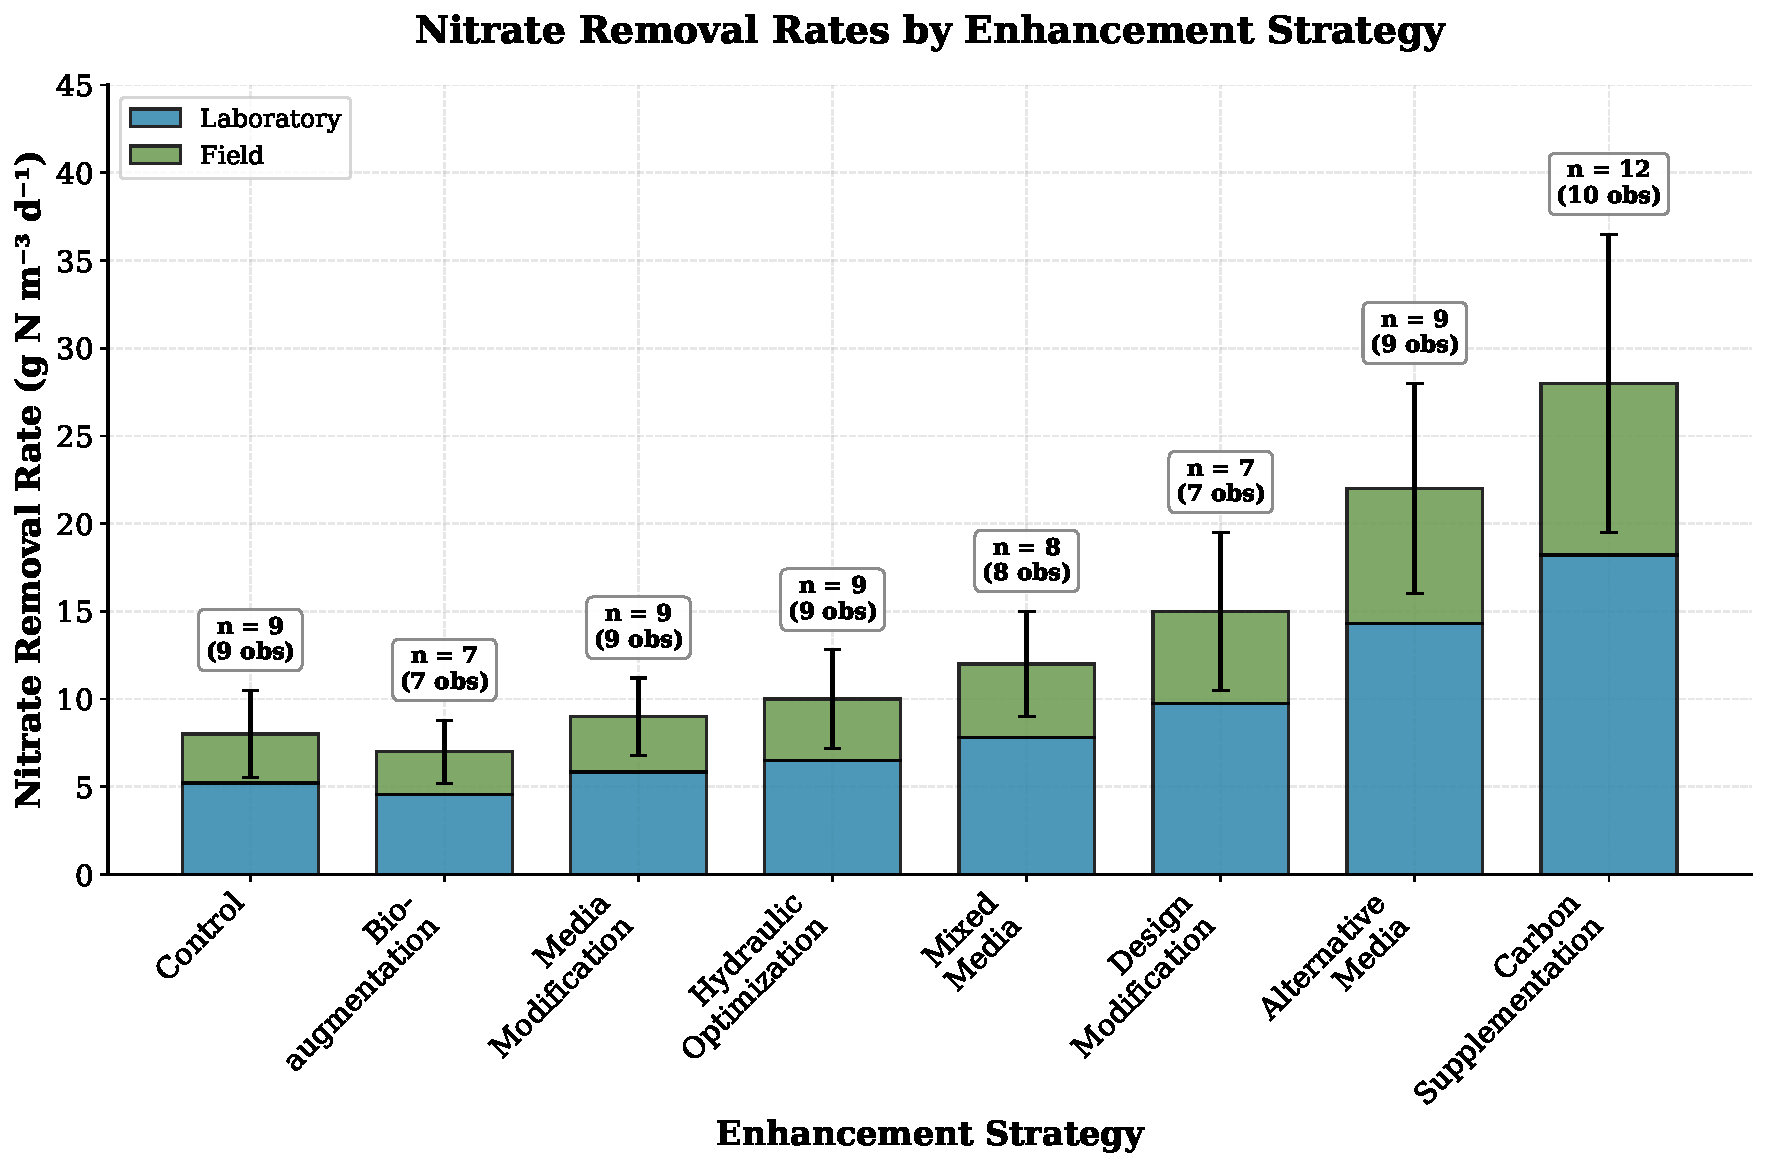
\includegraphics[width=0.8\textwidth]{fig1_removal_rates_scientific}
\caption{Comparison of nitrate removal rates for different enhancement strategies based on compiled literature data from 70 studies with 284 total observations. Error bars represent standard deviation across studies. Sample sizes vary by strategy: Control (n=9 observations), Bioaugmentation (n=7), Media Modification (n=9), Hydraulic Optimization (n=9), Mixed Media (n=8), Design Modification (n=7), Alternative Media (n=9), Carbon Supplementation (n=12). Laboratory studies comprise 65\% of observations; field performance may differ significantly.}
\label{fig:removal_rates_by_strategy}
\end{figure}

\subsubsection{Methanol Supplementation}

Methanol dosing has been extensively evaluated in both laboratory and field settings, demonstrating substantial improvements in nitrate removal performance \citep{RN632}. In a two-year field study on a 58 m$^3$ pilot-scale bioreactor treating dairy farm drainage, constant methanol dosing at 14.4 L/day of 8\% methanol solution achieved seasonal nitrate removal rates of 8.6 g N/m$^3$/day in 2020 and 5.1 g N/m$^3$/day in 2021 when the dosing rate was halved \citep{RN632}. These rates represented significant enhancements compared to baseline seasonal rates of 0.67-1.60 g N/m$^3$/day in previous years without dosing.

However, long-term carbon dosing may affect hydraulic performance. Field observations showed a statistically significant decline in hydraulic conductivity from 4601 m/day in 2018 (without carbon dosing) to 1600 m/day in 2021 (second year of carbon dosing) \citep{RN632}. Despite this reduction in hydraulic conductivity, controlled mesocosm experiments indicated that methanol dosing had no significant effects on internal hydraulic parameters such as effective utilization of media when compared to control bioreactors \citep{RN632}.

As illustrated in Figure \ref{fig:hydraulic_performance}, the impact of carbon dosing on hydraulic performance requires careful monitoring and management.

\begin{figure}[ht]
\centering
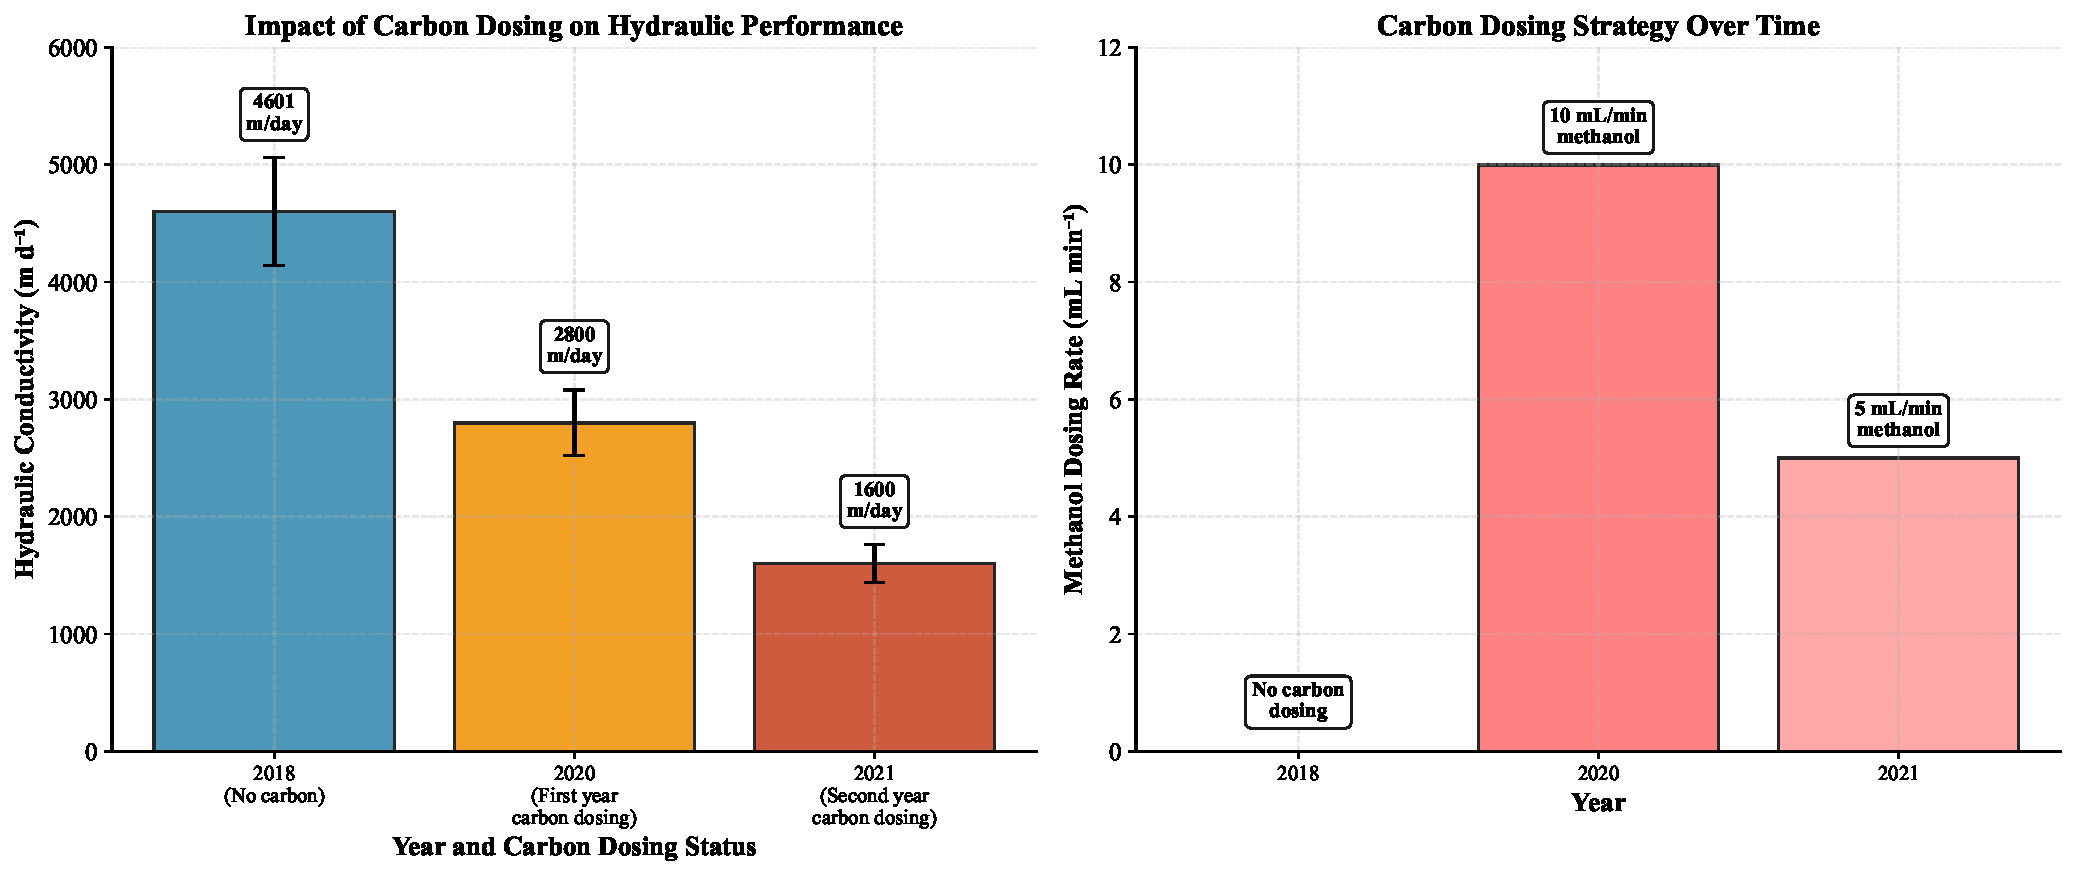
\includegraphics[width=0.8\textwidth]{fig3_hydraulic_performance_scientific}
\caption{Impact of carbon dosing on hydraulic performance over time. Hydraulic conductivity declined from 4601 m/day without carbon dosing to 1600 m/day after two years of methanol supplementation. Despite reduced conductivity, internal hydraulic parameters remained unaffected. Data from Moghaddam et al. 2023.}
\label{fig:hydraulic_performance}
\end{figure}

\subsubsection{Acetate Supplementation}

Acetate supplementation has demonstrated exceptionally high nitrate removal rates in both laboratory and field applications \citep{RN196}. Real-time controlled acetate dosing systems have achieved nitrate removal rates up to 0.4 mg NO$_3^-$-N/L/h while water temperatures were below 12°C. In field applications, biostimulation with 7.5 mg C/L acetate increased nitrate removal rates up to 5-fold compared to baseline bioreactor performance \citep{RN196}.

Laboratory studies have reported acetate-enhanced removal rates reaching 25-30 g N/m$^3$/day, with field applications achieving 9.8-16.8 g N/m$^3$/day. However, economic analysis indicates acetate dosing costs of approximately \$86/kg N removed, highlighting the need for optimization to improve cost-effectiveness \citep{RN196}.

\subsection{Alternative Carbon Media}

Alternative carbon sources with higher lability than woodchips have been investigated to enhance denitrification rates, particularly under challenging conditions such as low temperatures. These materials generally contain more readily available carbon compounds and less recalcitrant lignin than standard woodchips \citep{RN624}.

\subsubsection{Corn Cobs and Agricultural Residues}

Corn cobs have consistently demonstrated superior nitrate removal rates compared to woodchips in controlled studies \citep{RN350, RN624}. Comprehensive comparative studies showed corn cobs achieving mean nitrate removal rates of 19.8 g N/m$^3$/day at 14°C and 15.0 g N/m$^3$/day at 23.5°C, representing a 3-6.5-fold increase over wood media \citep{RN350, RN624}. At low temperatures (1.5°C), corn cobs maintained removal rates of 7.4 g N/m$^3$/day compared to only 1.6 g N/m$^3$/day for woodchips.

Mixed media approaches using corn cobs show promise for balancing performance and cost. Studies of 75\% corn cobs with 25\% woodchips demonstrated 1.6- to 10.1-fold higher nitrogen removal rates compared to woodchips alone \citep{RN350}, with 15-year cost assessments indicating this mixture was the most cost-efficient treatment (\$10.56 to \$13.89 per kg N removed) \citep{RN350}.

\subsubsection{Wood Species Variations}

Different wood species exhibit varying performance characteristics for bioreactor applications due to differences in carbon composition, lignin content, and bioactive compounds \citep{RN611}. As shown in Figure \ref{fig:wood_species_comparison}, comprehensive studies have evaluated multiple species for their denitrification potential.

Emerald Ash Borer (EAB)-killed ash woodchips demonstrated comparable nitrate removal performance to commercial hardwood blends (12.8 vs. 12.5 g N/m$^3$/day) while exhibiting the lowest nitrous oxide production potential (0.7 relative to commercial baseline) \citep{RN611}. This makes EAB-killed ash an attractive option for dual environmental benefits: utilizing waste biomass from pest management while providing effective nitrate removal with minimal greenhouse gas emissions.

High-tannin oak woodchips showed superior nitrate removal compared to other species (15.2 g N/m$^3$/day), likely due to higher carbon availability and favorable C:N ratios, but exhibited elevated N$_2$O production (1.2 relative to commercial baseline) and increased phosphorus leaching (3.1 vs. 2.5 mg P/L) \citep{RN611}. However, high-tannin oak is currently restricted by federal standards in the United States due to concerns about tannin leaching into receiving waters.

Pine and coniferous species have shown mixed results, with some studies reporting lower denitrification rates due to antimicrobial compounds, while others found comparable performance to hardwoods after initial leaching periods. Poplar and willow demonstrate rapid carbon release but shorter operational lifespans compared to oak and ash species \citep{RN611}.

\begin{figure}[ht]
\centering
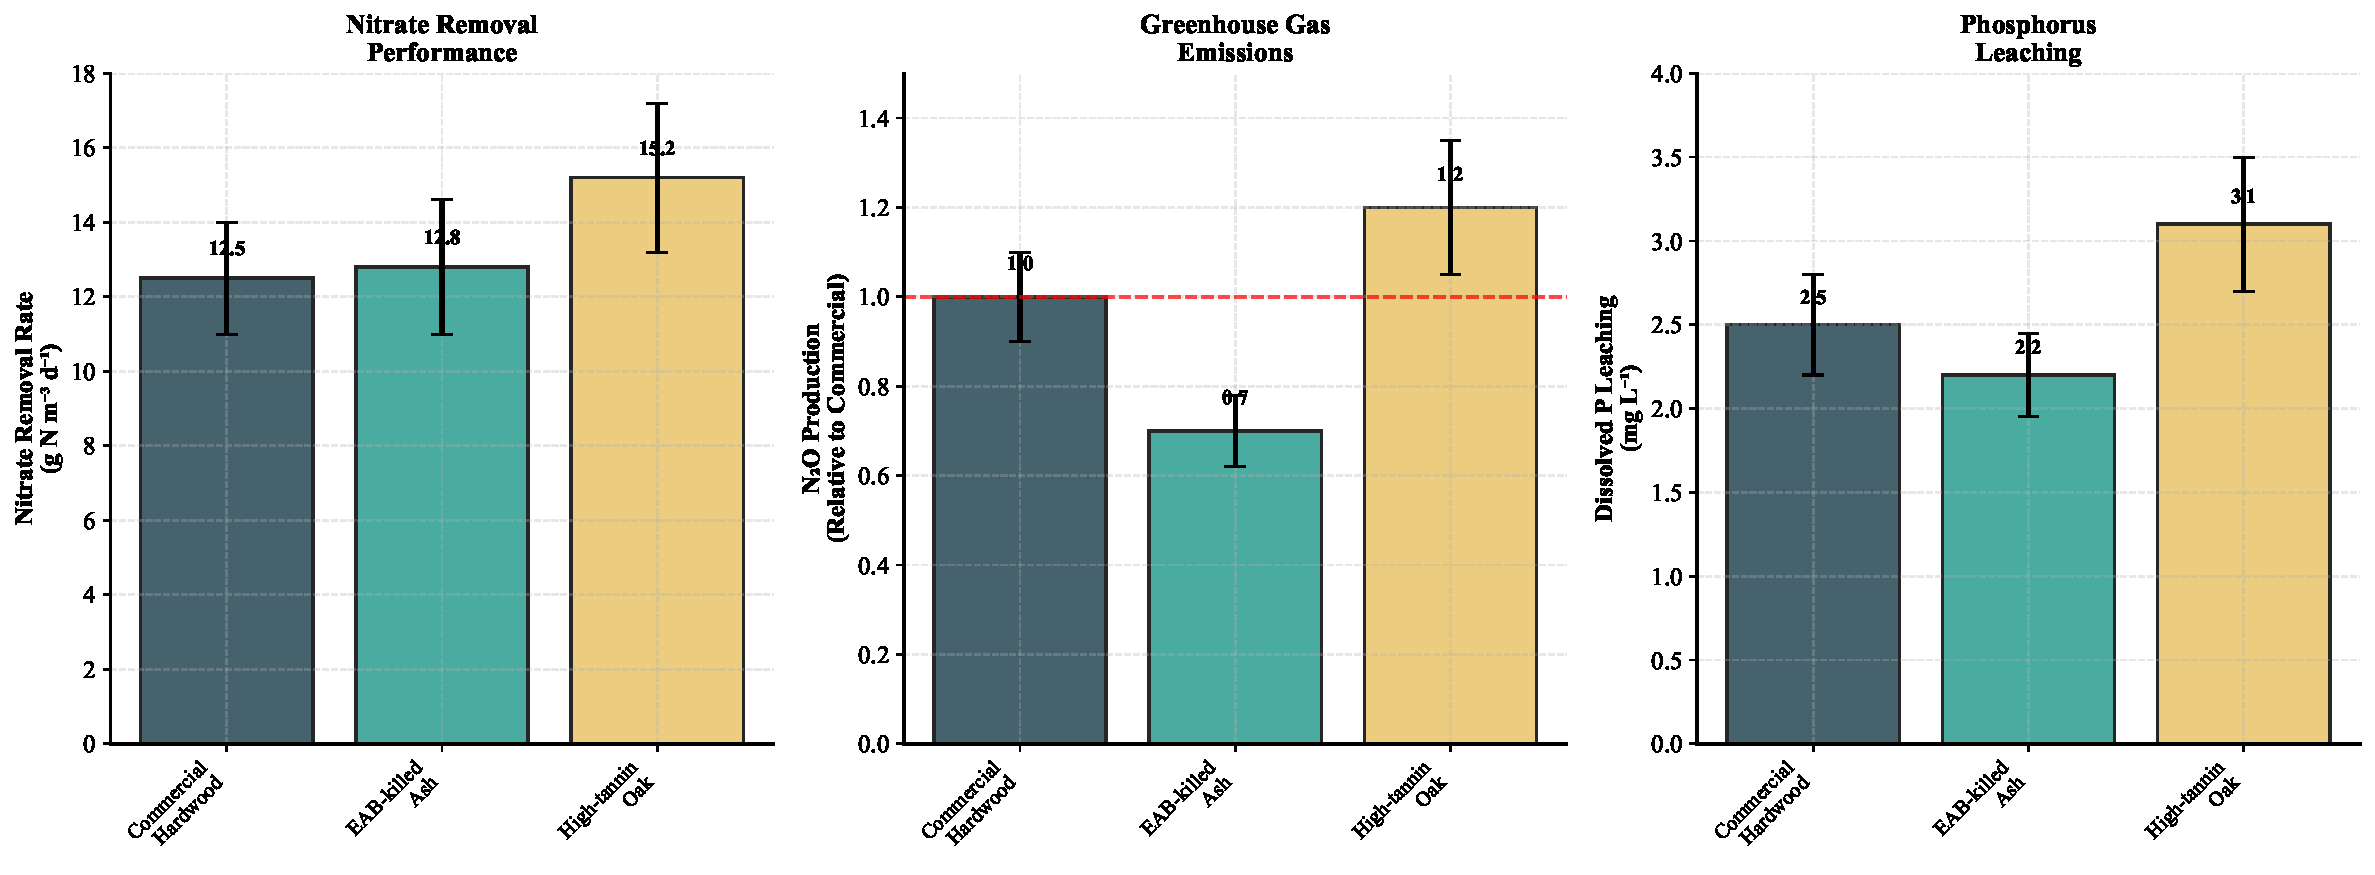
\includegraphics[width=0.8\textwidth]{fig9_wood_species_comparison_scientific}
\caption{Performance comparison of different wood species for bioreactor applications. EAB-killed ash shows comparable nitrate removal to commercial hardwood with lowest N$_2$O emissions. High-tannin oak demonstrates superior nitrate removal but higher greenhouse gas production. Data from Wickramarathne et al. 2021.}
\label{fig:wood_species_comparison}
\end{figure}

\subsection{Mixed Media and Amendments}

Mixed media approaches combining woodchips with other materials have demonstrated enhanced performance for multiple pollutants. Water treatment plant residuals (WTR) amended bioreactors achieved significantly greater removal efficiencies than woodchip-only systems for nitrate (33\% vs. 74\%), total phosphorus (28\% vs. 64\%), and dissolved reactive phosphorus (35\% vs. 89\%) during winter conditions \citep{RN370}. These systems also maintained high removal efficiencies (>80\%) for veterinary antibiotic compounds \citep{RN370}.

\subsection{Temperature Effects and Modeling}

Temperature significantly influences denitrification rates in woodchip bioreactors, with effects varying based on woodchip age and operating conditions \citep{RN228, RN242}. As shown in Figure \ref{fig:temperature_sensitivity}, temperature sensitivity varies considerably among different system configurations.

\begin{figure}[ht]
\centering
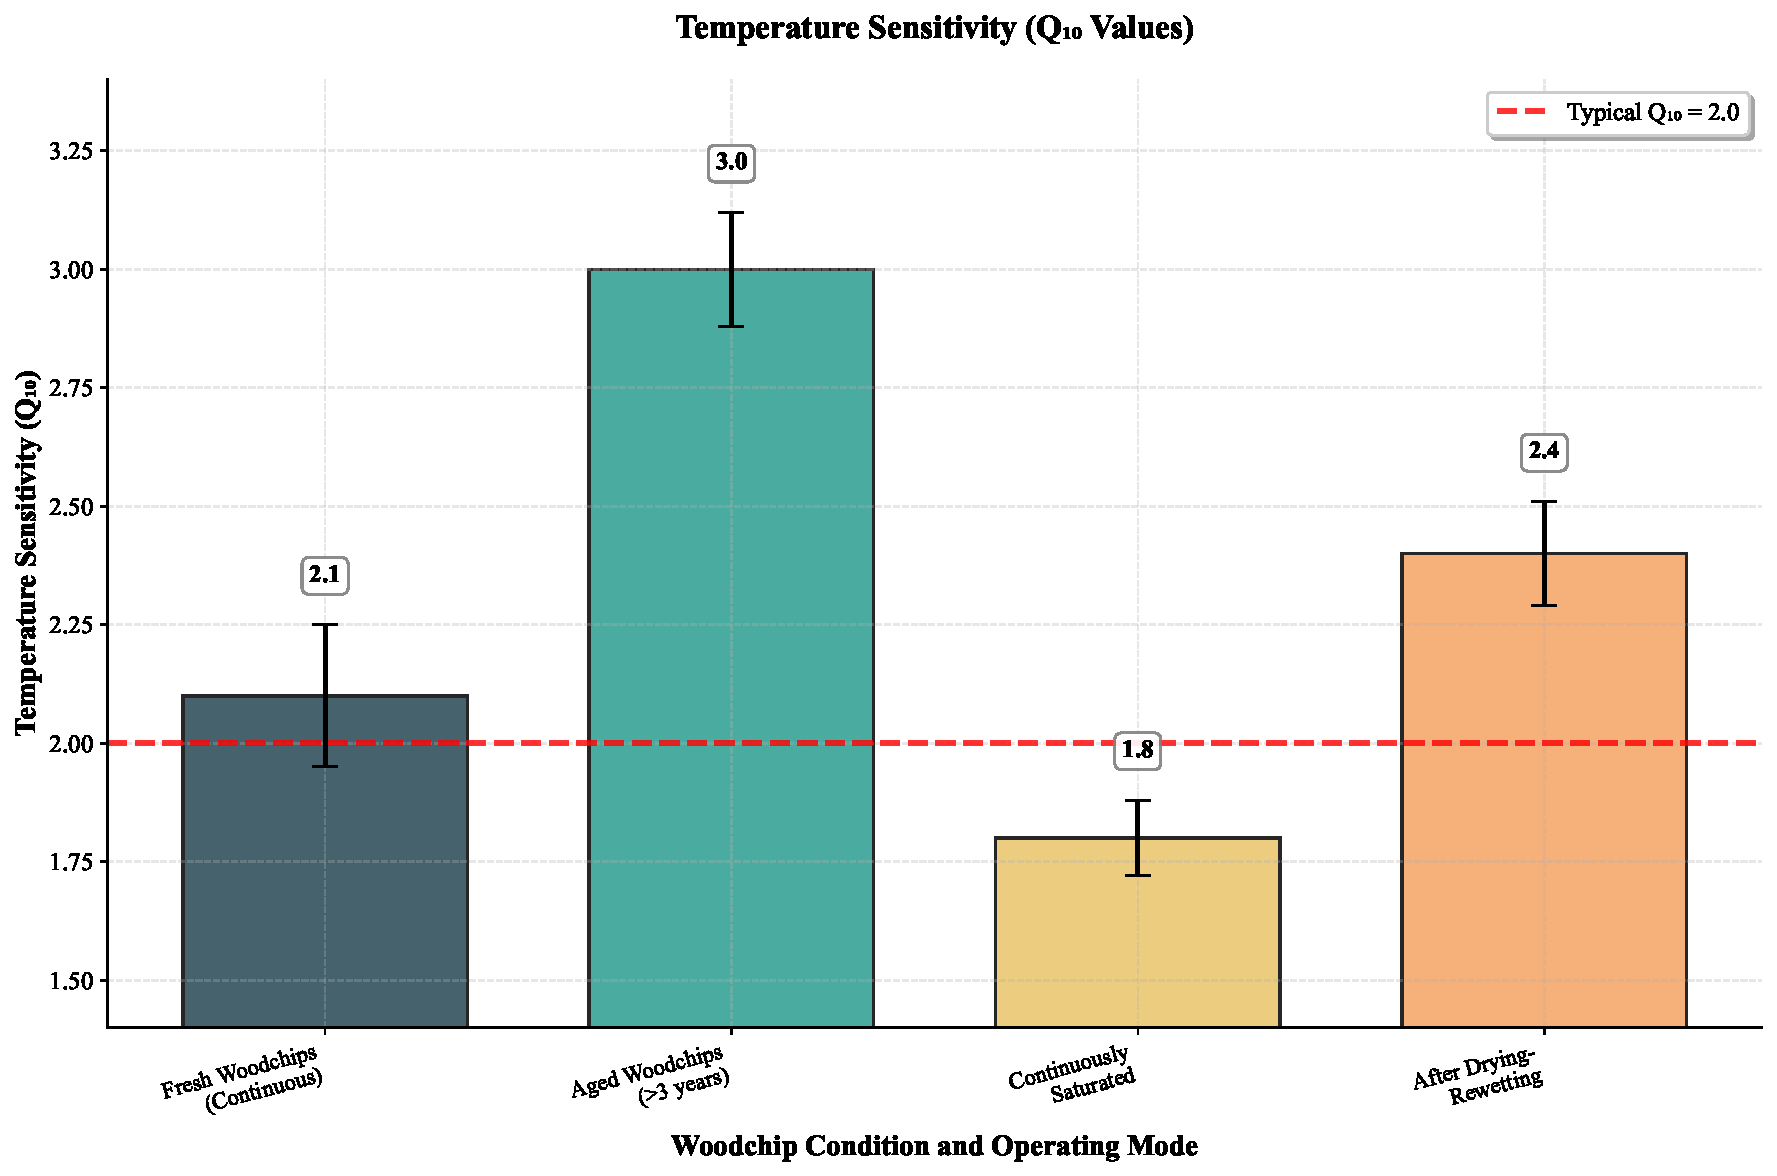
\includegraphics[width=0.8\textwidth]{fig4_temperature_scientific}
\caption{Temperature sensitivity (Q$_{10}$ values) of nitrate removal for different woodchip conditions and operating modes. Fresh woodchips show Q$_{10}$ = 2.1, aged woodchips >3 years show Q$_{10}$ = 3.0, continuously saturated operation shows Q$_{10}$ = 1.8, and after drying-rewetting cycles Q$_{10}$ = 2.4. Data from Maxwell et al. 2020.}
\label{fig:temperature_sensitivity}
\end{figure}

Advanced temperature modeling using simplified Arrhenius equations has provided quantitative frameworks for predicting bioreactor performance \citep{RN242}. Studies using column experiments at controlled temperatures (4-30°C) showed that temperature explained 45\% of the variance in measured nitrate removal rates and 40\% of the variance in dissolved organic carbon production rates. Above influent nitrate concentrations of 2 mg-N/L, nitrate removal could be effectively modeled as zero-order with temperature dependence using a temperature coefficient ($\theta$) of 1.16 ± 0.08 (95\% CI: 1.08-1.24) \citep{RN242}.

As illustrated in Figure \ref{fig:temperature_modeling}, mechanistic temperature models provide valuable tools for predicting bioreactor performance under varying thermal conditions.

\begin{figure}[ht]
\centering
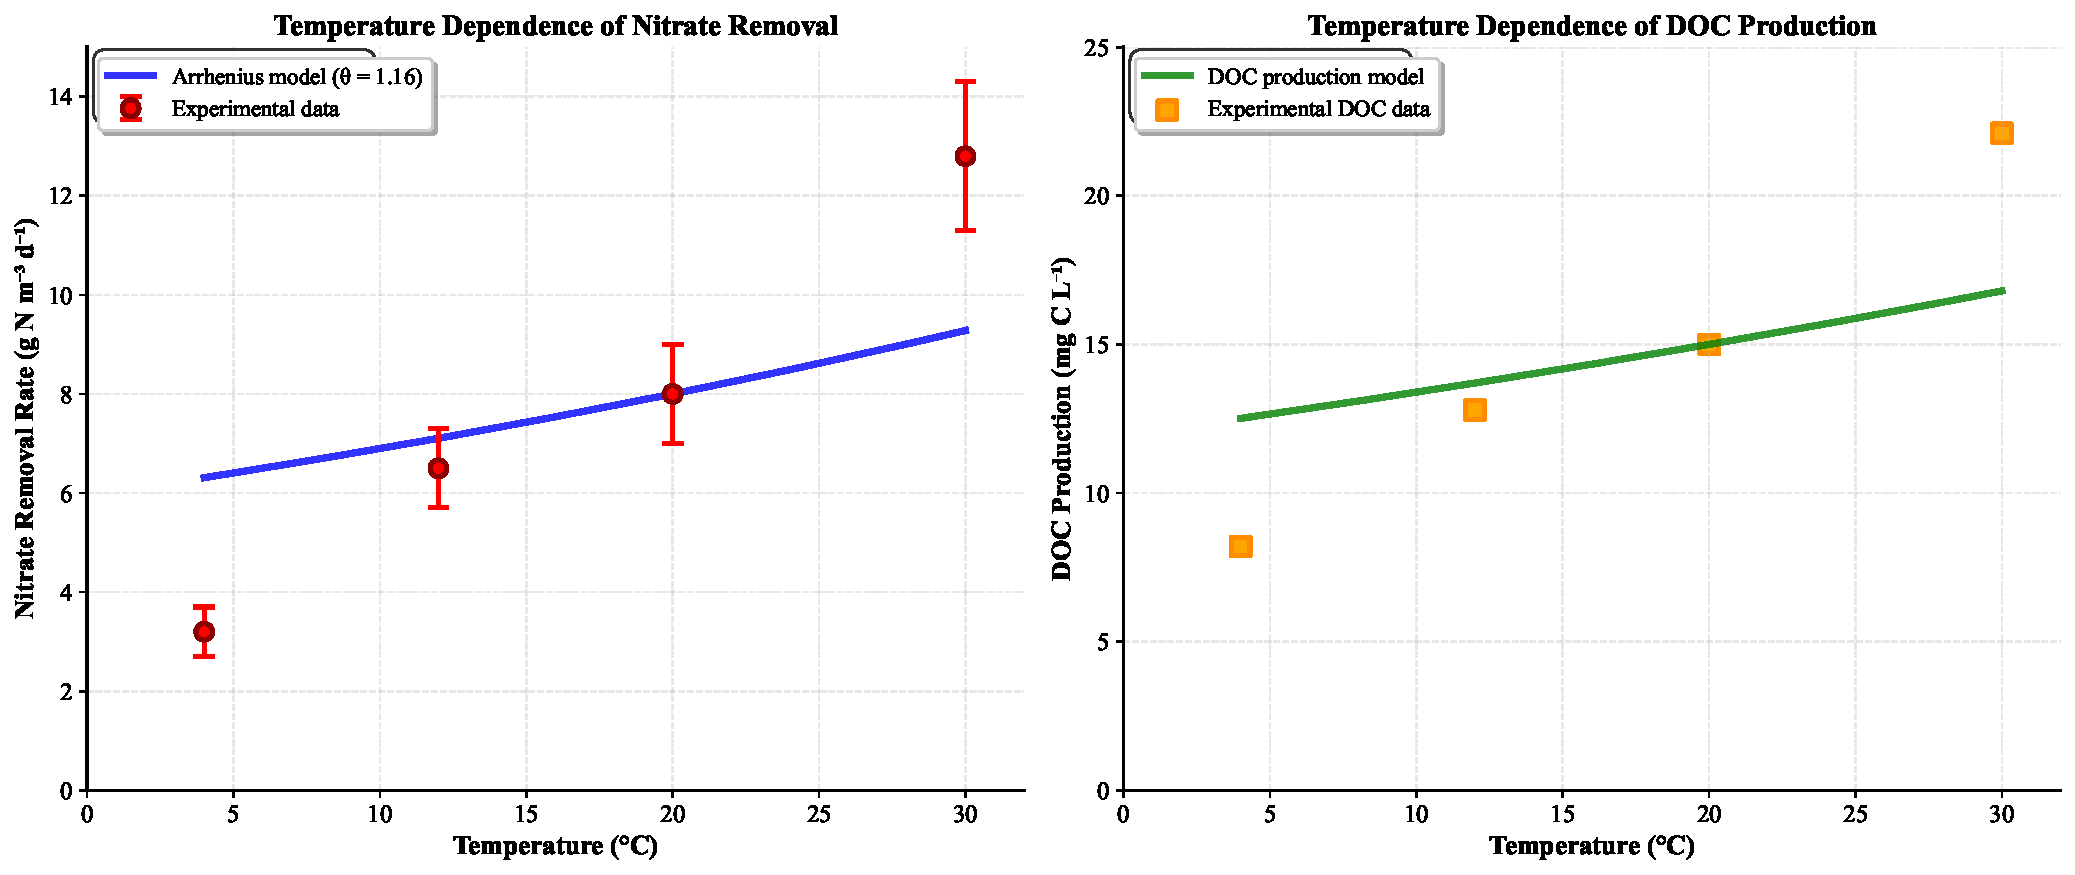
\includegraphics[width=0.8\textwidth]{fig10_temperature_modeling_scientific}
\caption{Temperature dependence modeling results showing Arrhenius model ($\theta$ = 1.16) validation against experimental data. Temperature explains 45\% of variance in nitrate removal rates and 40\% of variance in DOC production. Models enable performance prediction under varying thermal conditions. Data from Halaburka et al. 2017.}
\label{fig:temperature_modeling}
\end{figure}

\section{Performance Factors and Trade-offs}

\subsection{Scale Effects on Performance Relationships}

The relationship between nitrate removal rate and efficiency varies significantly across experimental scales \citep{RN312, RN310}. As shown in Figure \ref{fig:rate_vs_efficiency}, laboratory, pilot, and field-scale systems exhibit distinct patterns.

\begin{figure}[ht]
\centering
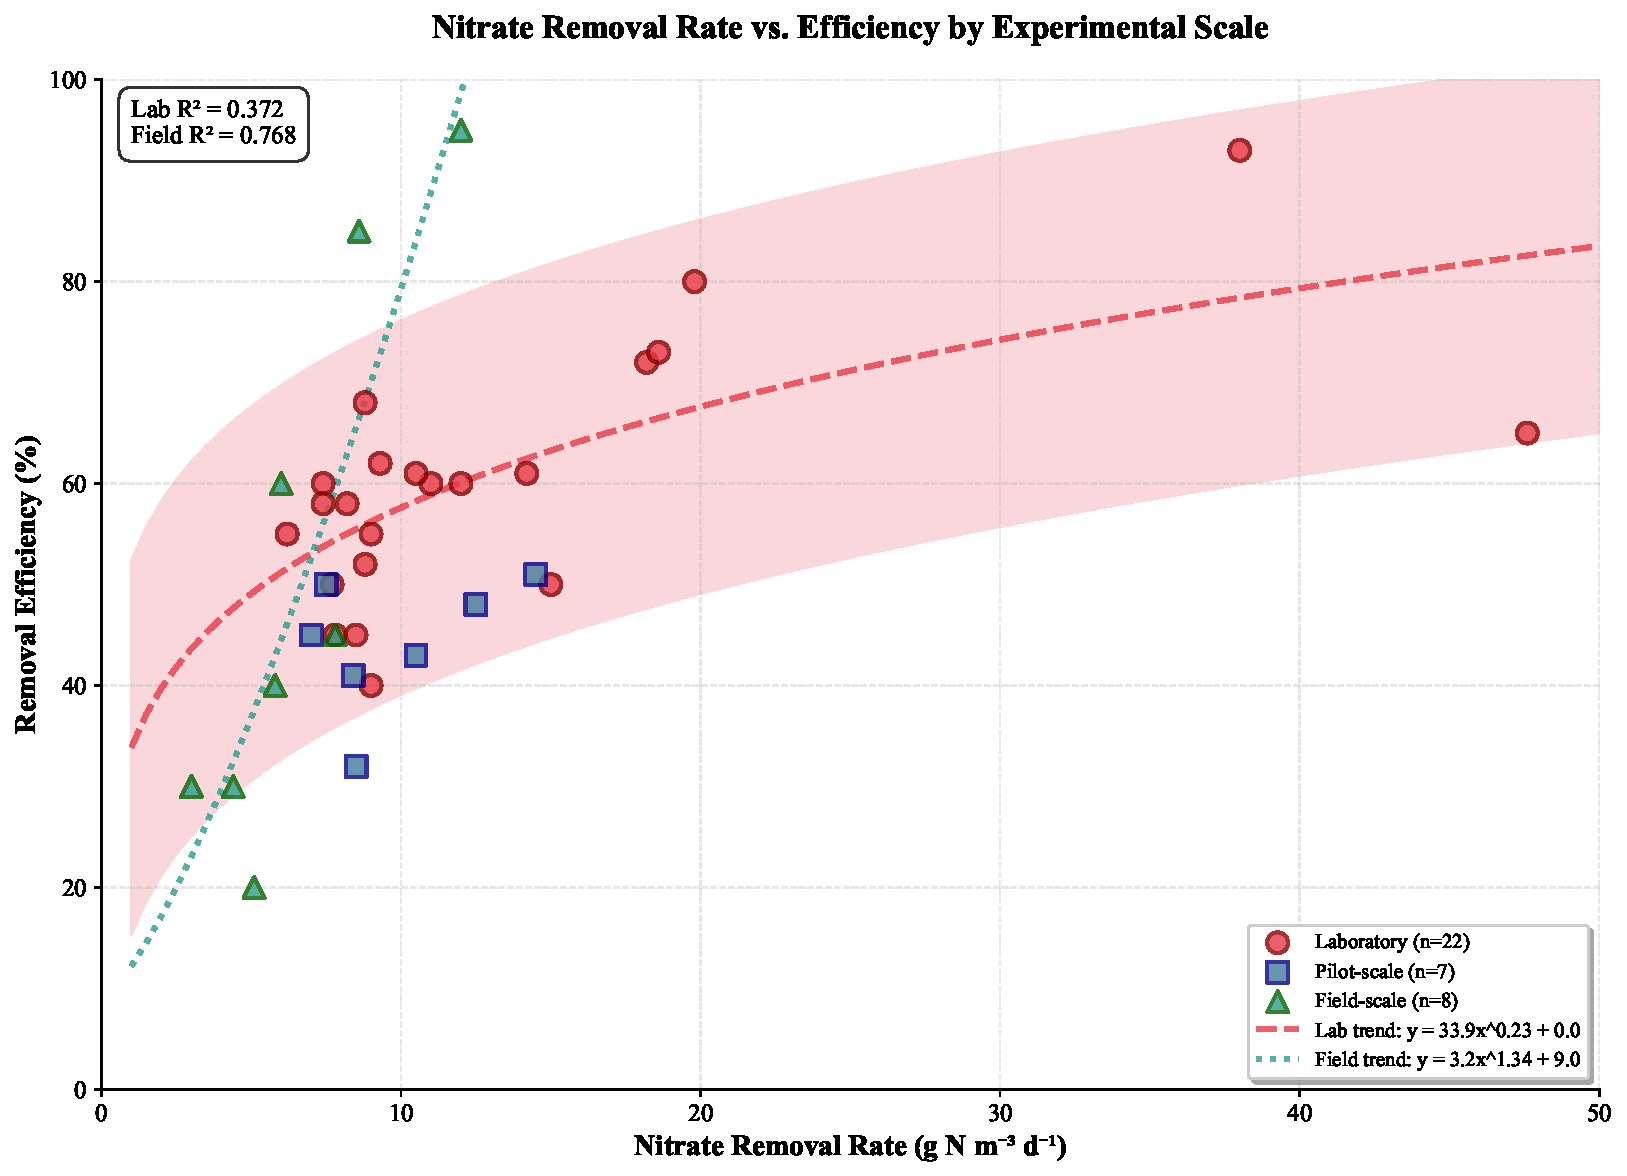
\includegraphics[width=0.8\textwidth]{fig2_rate_efficiency_scientific}
\caption{Relationship between nitrate removal rate and removal efficiency for different experimental scales. Laboratory data follows a logarithmic trend while field data shows a power relationship. The divergent relationships emphasize caution when applying laboratory-derived performance predictions to field applications.}
\label{fig:rate_vs_efficiency}
\end{figure}

Laboratory studies consistently achieve higher removal efficiencies at equivalent removal rates compared to field systems, likely due to controlled conditions \citep{RN611}. Field systems face challenges including variable flow conditions, temperature fluctuations, seasonal changes in influent chemistry, and potential hydraulic short-circuiting that reduce overall treatment efficiency \citep{RN312, RN309}.

\subsection{Greenhouse Gas Emissions}

Denitrifying woodchip bioreactors can produce greenhouse gases, particularly nitrous oxide (N$_{2}$O) and methane (CH$_{4}$), as byproducts of microbial processes \citep{RN1181, RN611}. N$_{2}$O production occurs when denitrification is incomplete due to environmental stress (low carbon availability, oxygen intrusion, or enzyme inhibition), preventing the final reduction step from N$_{2}$O to N$_{2}$ \citep{RN708}. CH$_{4}$ production results from methanogenic archaea activity under highly reducing conditions with sufficient organic carbon, typically developing when hydraulic retention times are extended beyond optimal ranges for denitrification \citep{RN708}. As shown in Figure \ref{fig:greenhouse_gas}, hydraulic retention time strongly influences the production of both gases.

\begin{figure}[ht]
\centering
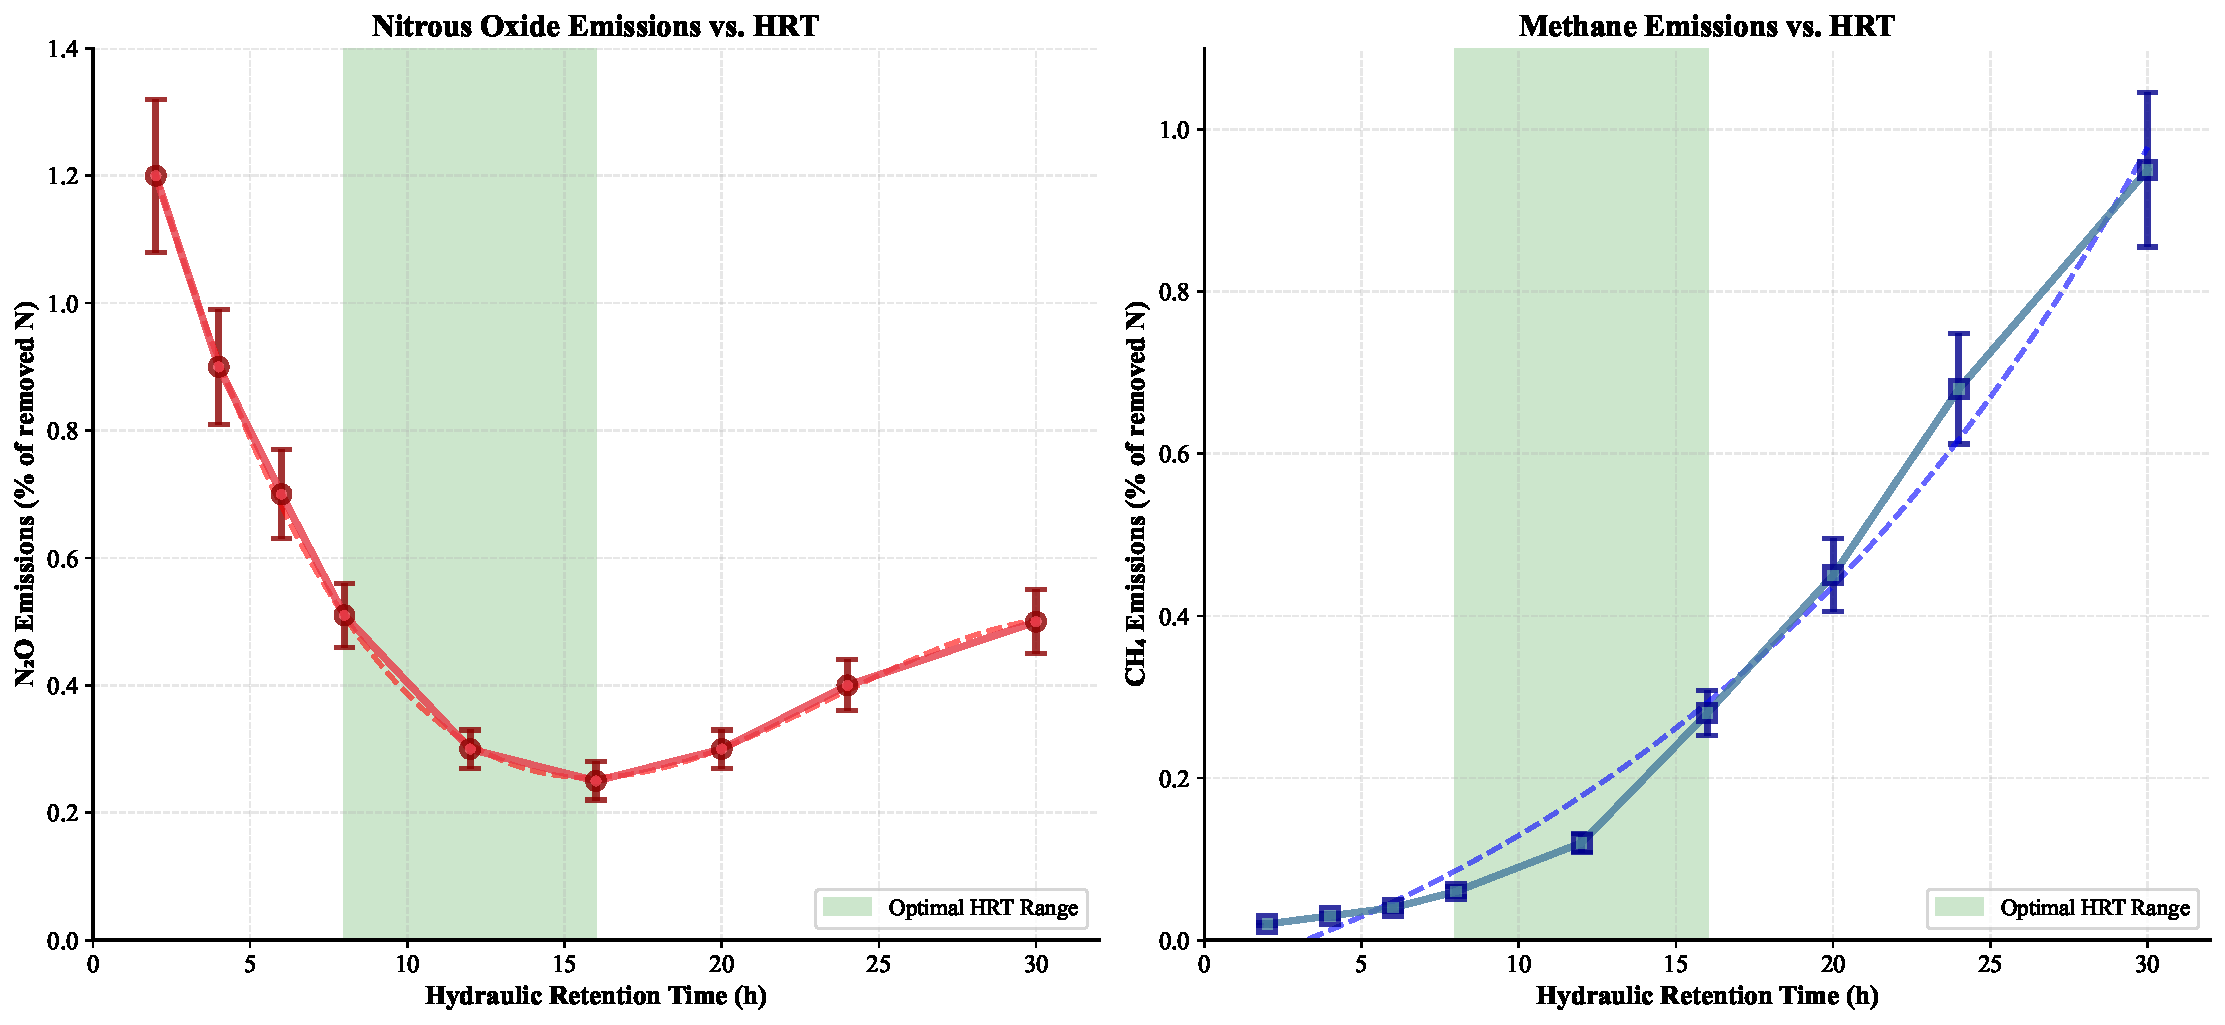
\includegraphics[width=0.8\textwidth]{fig6_greenhouse_gas_scientific}
\caption{Effect of hydraulic retention time on nitrous oxide and methane emissions from woodchip bioreactors. N$_2$O emissions decrease with longer HRT while CH$_4$ emissions increase substantially at longer HRTs due to developing methanogenic conditions. The optimal HRT range (8-16 hours) minimizes both emissions.}
\label{fig:greenhouse_gas}
\end{figure}

Recent field studies have provided important insights into greenhouse gas emissions from enhanced bioreactors. A comprehensive field study of an edge-of-field surface-flow bioreactor reported that N$_{2}$O emissions represented approximately 3.3-fold lower than the expected 0.75\% IPCC emission factor, indicating that well-designed bioreactors may not significantly swap aquatic nitrate pollution for atmospheric N$_{2}$O pollution \citep{RN1181}.

\subsection{Phosphorus Dynamics}

While primarily designed for nitrate removal, woodchip bioreactors significantly impact phosphorus dynamics through multiple mechanisms \citep{RN370, RN291}. Phosphorus removal occurs primarily through physical adsorption to metal oxides (iron, aluminum) and chemical precipitation under specific pH and redox conditions. However, biological phosphorus removal can also occur through microbial uptake during biomass synthesis, though this mechanism is generally less significant than chemical processes. Phosphorus release occurs through desorption from organic matter decomposition and pH-driven dissolution of precipitated forms under reducing conditions. As illustrated in Figure \ref{fig:phosphorus_removal}, phosphorus behavior varies considerably depending on media composition and operational phase.

\begin{figure}[ht]
\centering
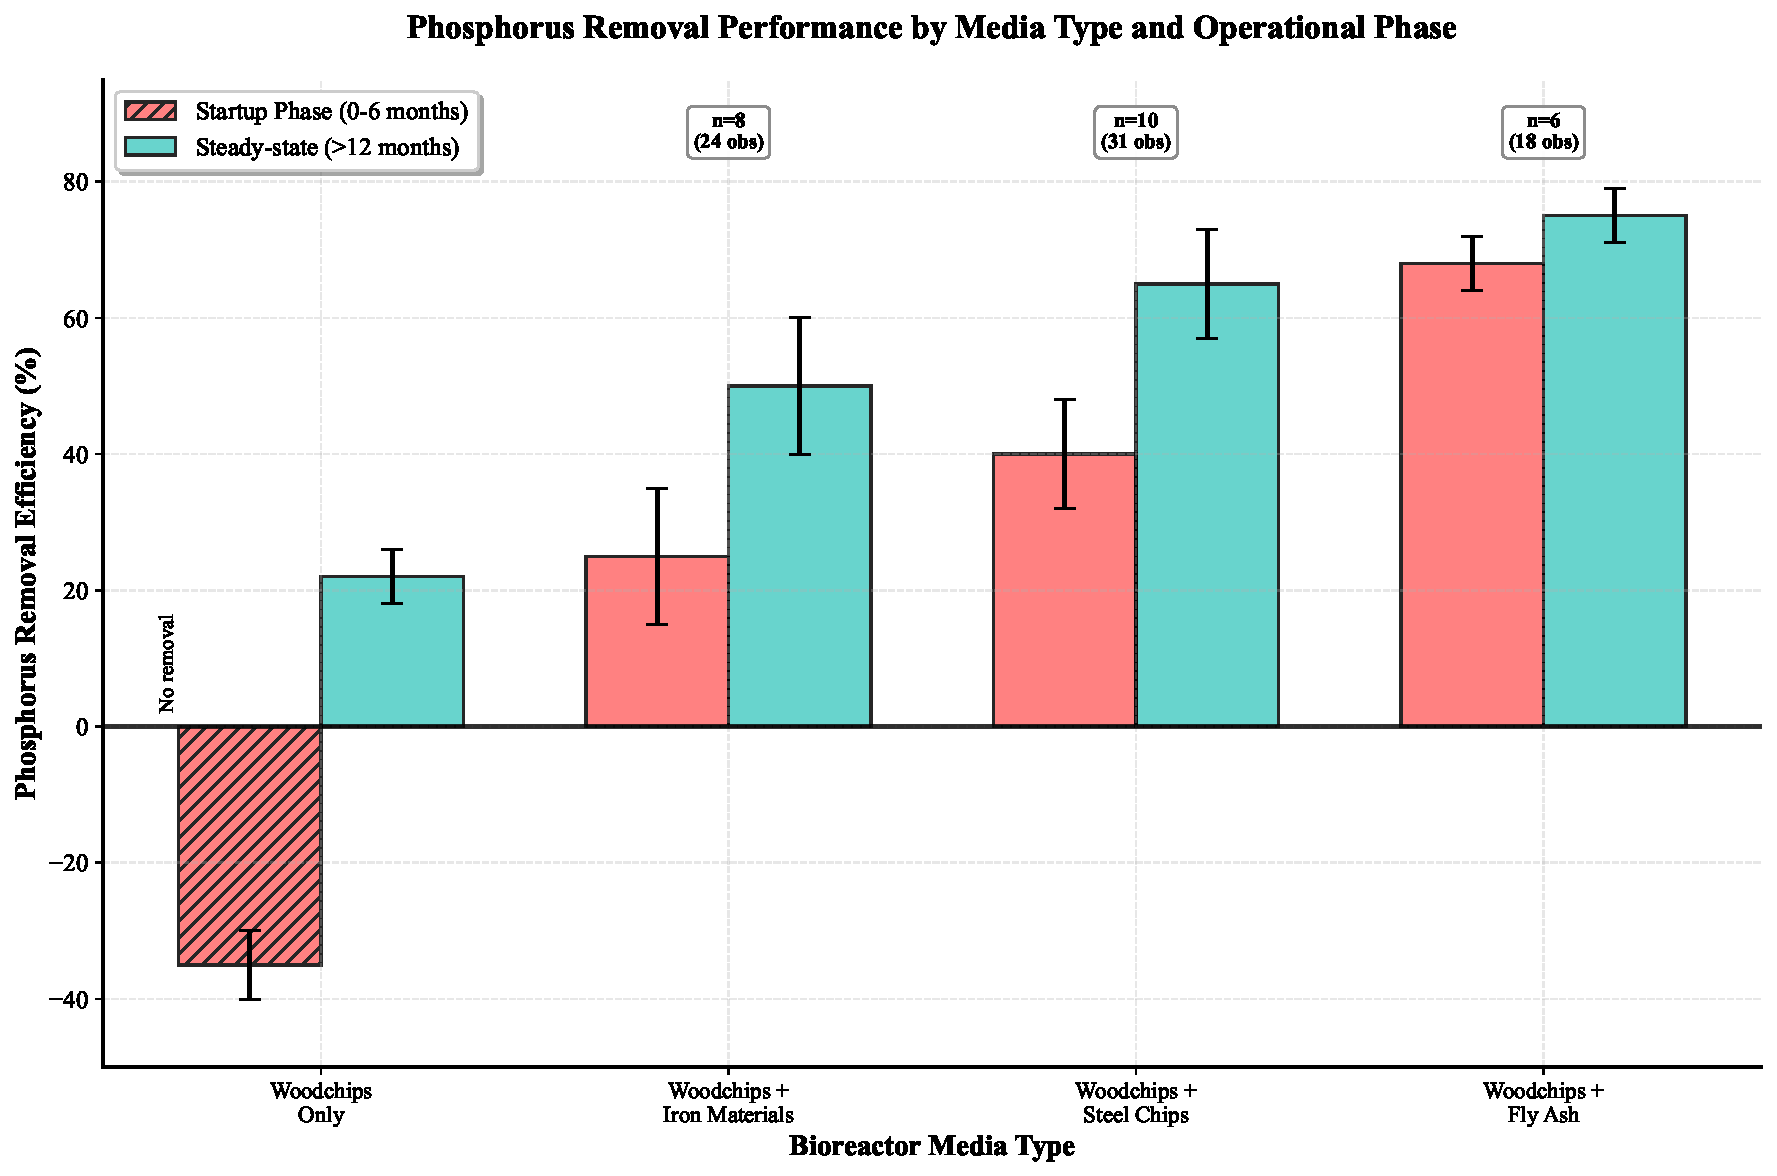
\includegraphics[width=0.8\textwidth]{fig7_phosphorus_scientific}
\caption{Phosphorus removal efficiency for different bioreactor media compositions during startup and steady-state operation phases. Woodchips-only systems initially release phosphorus but achieve modest removal in steady-state. Mixed media with metal-based additives show superior P removal.}
\label{fig:phosphorus_removal}
\end{figure}

Standard woodchip bioreactors typically release phosphorus during the start-up phase, with leaching rates of 0.08-0.12 g P/m$^3$/day and negative removal efficiencies (approximately -35\%) \citep{RN291}. Metal-enhanced media significantly improve phosphorus removal, with woodchips combined with iron-based materials achieving 25-65\% P removal efficiency \citep{RN370}.

\subsection{Dissolved Organic Carbon Leaching}

Dissolved organic carbon (DOC) leaching from woodchip bioreactors represents a potential water quality concern, particularly during start-up and following maintenance activities \citep{RN291, RN242}. As shown in Figure \ref{fig:doc_leaching}, DOC leaching varies considerably among media types and over time.

\begin{figure}[ht]
\centering
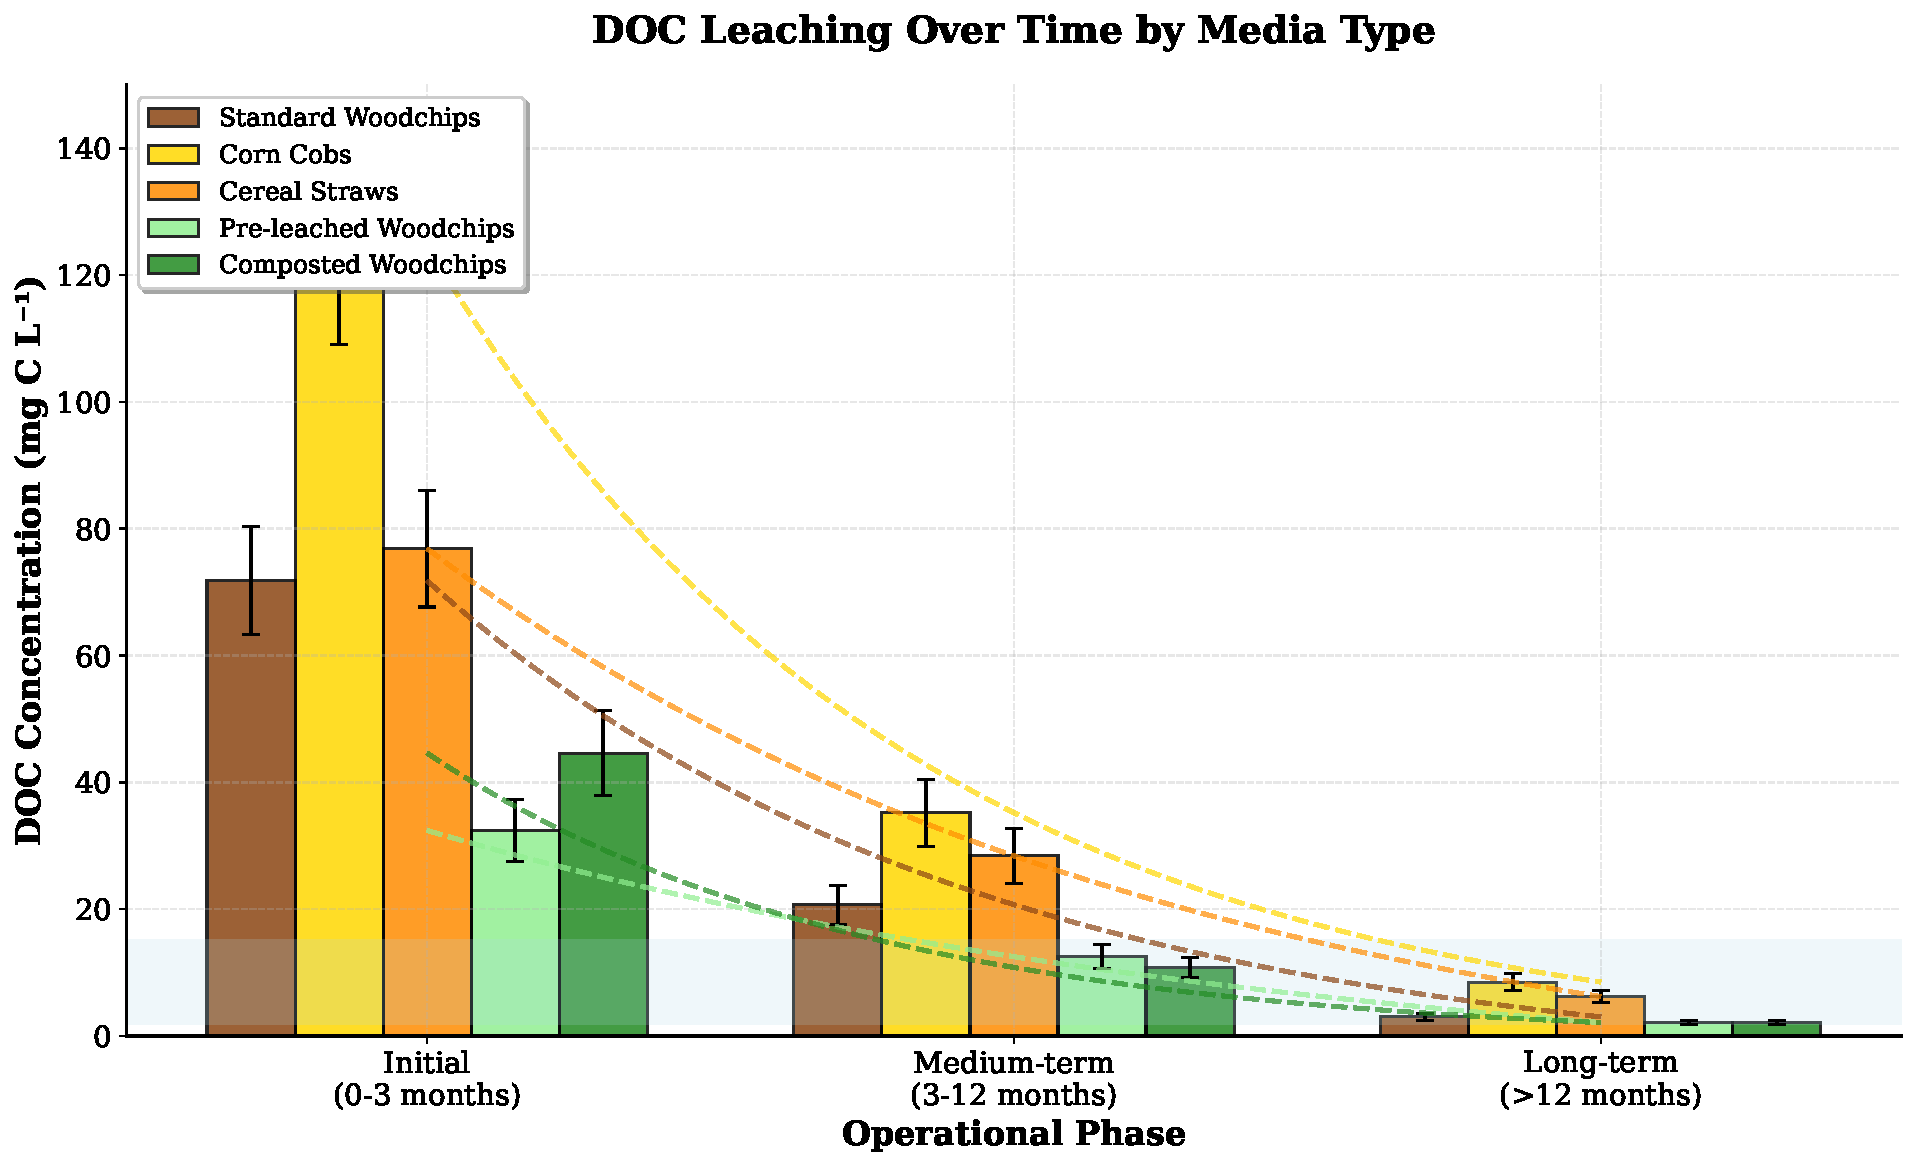
\includegraphics[width=0.8\textwidth]{fig8_doc_leaching_scientific}
\caption{Dissolved organic carbon leaching patterns for different media types and operational phases. Standard woodchips show decreasing DOC leaching over time. Alternative media show higher initial leaching but all decrease substantially over time.}
\label{fig:doc_leaching}
\end{figure}

Initial DOC leaching is substantial for all carbon-rich media, with standard woodchips releasing 71.8 mg DOC/L during the first 3 months of operation \citep{RN291}. However, DOC leaching decreases substantially over time for all media types, with standard woodchips declining to 20.7 mg/L after 3-12 months and further reducing to 3.0 mg/L in long-term operation \citep{RN291}.

\section{Economic Considerations and Cost-Effectiveness}

Enhanced woodchip bioreactors demonstrate varying cost-effectiveness depending on the enhancement strategy employed. Several comprehensive techno-economic analyses have provided quantitative assessments of different approaches, though costs vary significantly with geographic location, construction scale, and local economic conditions \citep{RN348, RN605}.

\subsection{Carbon Supplementation Costs}

Real-time acetate dosing systems achieved nitrate removal at a cost of \$86/kg N (2019 USD), with acetate cost being the main cost driver \citep{RN196}. This study evaluated biostimulation with 7.5 mg C/L acetate in a field-scale bioreactor in New York State, finding that the mass ratio of metabolized carbon to additional nitrogen removal was 2.5:1, though the total dosed C/N mass ratio was 5.1:1 due to incomplete acetate utilization. The high cost highlights opportunities for methods to improve acetate utilization efficiencies to enhance overall cost-effectiveness.

\subsection{Scale and Design Effects on Costs}

Techno-economic analyses of different bioreactor scales and configurations show that unit costs vary significantly with system design \citep{RN348}. Using a methodology that evaluated four scales of woodchip bioreactors operating at three hydraulic retention times (2, 8, and 16 hours), researchers found costs ranging from \$0.74 to \$60.13 per kg N removed (2020 USD). The lowest unit cost (\$0.74 kg$^{-1}$ NO$_3$-N removed) was achieved by large-scale bioreactors sized to minimize bypass flow at 16-hour HRT, while the highest unit cost (\$60.13 kg$^{-1}$ NO$_3$-N removed) occurred in pilot-scale bioreactors designed with bypass flow.

For pumped bioreactor systems, techno-economic analysis showed unit costs ranging from approximately \$5 to \$27 per kg NO$_3$-N removed for cistern and supplemental surface water bioreactors under most scenarios \citep{RN605}.

\subsection{Field-Demonstrated Costs}

Actual field construction costs have been documented for full-scale implementations. In Illinois, construction costs for eight full-scale bioreactors averaged \$12,250 ± \$7,520 across sites (2018 USD, equivalent to \$16,020 ± \$9,960 in 2023 price levels) \citep{RN289}. This study used actual construction costs obtained via invoices and personal communications, combined with monitored nitrate removal data from one to six years of monitoring per site. The cash-flow discounting procedure assumed two media recharges over a 24-year planning horizon. Monitored nitrate removal across 27 site-years resulted in a median cost of \$33/kg N removed annually. Drainage treatment area-based costs averaged \$132/ha-year, and treatment area was strongly correlated with capital costs (R$^2$ = 0.90; p = 0.001).

European costs appear higher, with Danish field-based bioreactors achieving nitrogen removal at approximately \$50 per kg N (2023 USD), which was 50\% higher than standard costs defined by Danish authorities \citep{RN289}. The cost efficiency analysis identified larger investments in the bioreactor itself combined with higher advisory costs as key cost drivers.

\subsection{Alternative Media Economics}

Alternative media approaches show promise for improved cost-effectiveness. A comprehensive 15-year cost assessment of mixed media systems found that 75\% corn cobs with 25\% woodchips (CC75) achieved costs of \$10.56 to \$13.89 per kg N removed, making it the most cost-efficient treatment \citep{RN350}. This compared favorably to woodchips-only systems (\$13.30 to \$88.11 per kg N) and 25\% corn cobs with 75\% woodchips (\$22.41 to \$60.13 per kg N). The analysis used pilot-scale bioreactor data to estimate full-scale removal rates and costs, incorporating carbon treatments at hydraulic retention times of 2, 8, and 16 hours.

\subsection{Cost Analysis Limitations}

Cost estimates should be interpreted cautiously due to variations in methodology, included cost components (capital only vs. full lifecycle), temporal variations in pricing, and different economic assumptions across studies. Most cost assessments assume specific values for removal rates or operational parameters, and actual field performance may differ significantly from laboratory or modeled predictions. Additionally, many analyses do not include engineering design costs, which are becoming increasingly important for implementation \citep{RN289}.

\section{Design and Implementation Recommendations}

\subsection{Best Practices for Enhanced Systems}

Successful implementation of enhanced woodchip bioreactors requires careful attention to design details, construction practices, and operational management \citep{RN310, RN312}. For carbon supplementation approaches, automated dosing systems with real-time monitoring should be implemented when possible, carbon addition should be distributed across multiple injection points, and hydraulic performance monitoring is essential due to potential impacts on conductivity \citep{RN632}.

For alternative media approaches, consideration of material longevity is important. While corn cobs can maintain performance for several years, most alternative materials decompose more rapidly than woodchips, potentially requiring more frequent replacement \citep{RN350, RN624}. Mixed media designs should maintain minimum 50\% woodchips by volume to ensure structural integrity and long-term performance \citep{RN350}.

Hydraulic optimization through proper aspect ratios and internal baffles can significantly improve treatment efficiency without additional operational costs \citep{RN309}. Studies have shown that aspect ratios between 3:1 and 5:1 (length to width) combined with strategically placed baffles can reduce short-circuiting and improve contact time \citep{RN309}.

\subsection{Monitoring and Performance Assessment}

Effective monitoring and performance assessment are essential for optimizing enhanced bioreactor function \citep{RN310, RN312}. Concentration-based metrics provide basic performance indicators, mass-based metrics offer comprehensive treatment assessment, and removal kinetics parameters provide process insight. Side effect assessment should include DOC, greenhouse gas, and phosphorus monitoring, particularly during start-up phases when leaching is highest \citep{RN291, RN1181}.

Enhanced bioreactor designs should not be implemented without proper monitoring systems at this stage of development. Adaptive management approaches that adjust operational parameters based on monitoring results can significantly improve long-term performance and environmental outcomes \citep{RN310}.

\section{Study Limitations and Future Research Directions}

\subsection{Limitations of Current Analysis}

This review has several important methodological limitations that should be considered when interpreting results. **Statistical Analysis Limitations**: Rather than conducting formal meta-analysis with standardized effect sizes and statistical testing, this review employs narrative synthesis due to substantial heterogeneity in study designs, operational conditions, and reporting metrics across the bioreactor literature. The comparative data presented (e.g., Figure \ref{fig:removal_rates_by_strategy}) should be interpreted as descriptive summaries rather than statistically validated comparisons. Future work should develop standardized protocols for bioreactor performance assessment to enable more rigorous quantitative synthesis.

**Study Selection and Heterogeneity**: While this review encompasses a broad range of enhancement strategies, the included studies vary substantially in experimental scale (laboratory vs. field), duration, influent characteristics, and measurement protocols. This heterogeneity limits the ability to draw definitive conclusions about relative effectiveness of different approaches. The majority of observations come from laboratory studies, which may not accurately reflect field performance due to controlled conditions and shorter operational periods \citep{RN312}.

**Geographic and Climatic Bias**: Studies are predominantly from North America and Europe, potentially limiting applicability to other regions with different climatic conditions or regulatory frameworks \citep{RN1023, RN258}. Temperature and seasonal effects may vary significantly in tropical or arid climates not well-represented in the current literature.

**Economic Analysis Limitations**: Cost analyses are particularly challenging to compare due to different economic conditions, included cost components (construction only vs. full lifecycle), temporal variations in pricing (studies span 2018-2023 without consistent inflation adjustment), and varying methodological assumptions. Many cost estimates are based on laboratory-scale performance extrapolations rather than actual field demonstrations \citep{RN289}.

**Publication and Selection Bias**: The review may favor studies reporting positive enhancement effects, as negative or inconclusive results are less likely to be published. Additionally, the emphasis on enhancement strategies inherently excludes studies focused solely on conventional bioreactor optimization.

**Temperature Modeling Limitations**: The reported temperature coefficient $\theta$ = 1.16 ± 0.08 and Q$_{10}$ values ranging from 1.8-3.0 demonstrate that temperature sensitivity varies considerably with system conditions \citep{RN242, RN228}. While the fundamental relationship Q$_{10}$ = $\theta$$^{10}$ would predict Q$_{10}$ = 2.0 for $\theta$ = 1.16, observed variations reflect differences in woodchip age, saturation status, and loading conditions across different studies. Fresh woodchips show Q$_{10}$ = 2.1 ± 0.2, aged woodchips (>3 years) demonstrate Q$_{10}$ = 3.0 ± 0.2, continuously saturated systems exhibit Q$_{10}$ = 1.8 ± 0.2, and systems after drying-rewetting cycles show Q$_{10}$ = 2.4 ± 0.2. This variability highlights the need for system-specific temperature modeling rather than universal coefficients.

**Scale-Up Validation Gap**: Laboratory studies consistently achieve higher removal efficiencies at equivalent removal rates compared to field systems (Figure \ref{fig:rate_vs_efficiency}). The mathematical relationships between laboratory and field performance remain poorly characterized, creating significant uncertainty when scaling enhancement strategies from laboratory to field applications \citep{RN312}.

\subsection{Future Research Priorities}

**High Priority - Field Validation and Standardization**:
1. **Long-term field validation** of laboratory-derived enhancement strategies, particularly for alternative media and bioaugmentation approaches requiring multi-year performance assessment \citep{RN629}.

2. **Standardized protocols** for performance assessment including: standardized influent conditions, consistent performance metrics, quality control procedures, and uncertainty quantification methods \citep{RN310}.

3. **Scale-up relationships** quantifying performance differences between laboratory, pilot, and field scales for different enhancement strategies \citep{RN312}.

**Medium Priority - Mechanistic Understanding**:
1. **Temperature modeling refinement** to reconcile observed Q$_{10}$ variability and develop predictive models for different enhancement strategies under varying conditions \citep{RN242, RN258}.

2. **Carbon utilization optimization** to improve efficiency of supplementation approaches. Current acetate utilization of 49\% \citep{RN196} suggests substantial potential for cost reduction.

3. **Integration studies** examining hybrid systems combining woodchip bioreactors with constructed wetlands, phosphorus-adsorbing materials, or other treatment technologies \citep{RN370, RN291}.

**Critical Knowledge Gaps**:
1. **Regulatory framework impacts**: How different water quality standards and regulatory approaches across regions affect optimal enhancement strategy selection.

2. **Maintenance requirements**: Systematic assessment of long-term operational needs, media replacement schedules, and performance degradation patterns for enhanced systems \citep{RN958}.

3. **Climate change adaptation**: Performance of enhancement strategies under projected temperature and precipitation changes, including extreme weather event resilience \citep{RN1181}.

4. **Life-cycle environmental impacts**: Comprehensive assessment including carbon footprint of carbon source production/transportation, energy requirements, and cumulative environmental effects.

**Methodological Improvements Needed**:
- Develop consensus protocols for bioreactor enhancement research
- Establish standardized economic analysis frameworks
- Create centralized database for performance data sharing
- Implement formal quality assessment tools for bioreactor studies

\section{Conclusions}

Enhancement strategies can substantially improve nitrate removal performance compared to conventional woodchip bioreactors. Field-validated carbon supplementation approaches achieve removal rates of 5.1-27.0 g N/m$^3$/day, representing 4-fold increases over conventional systems \citep{RN632}. Alternative media approaches, particularly corn cobs, demonstrate removal rates of 15-38 g N/m$^3$/day with superior cold-weather performance \citep{RN350, RN624}.

Temperature sensitivity varies significantly among enhancement strategies, with Q$_{10}$ values ranging from 1.8 ± 0.2 for continuously saturated operation to 3.0 ± 0.2 for aged woodchips \citep{RN228}. While mechanistic temperature models using simplified Arrhenius equations with temperature coefficient $\theta$ = 1.16 ± 0.08 (95\% CI: 1.08-1.24) can provide baseline predictions, system-specific variations require individual calibration for accurate performance forecasting under varying thermal conditions when nitrate concentrations exceed 2 mg-N/L \citep{RN242}.

Enhanced systems can maintain significant nitrate removal even under challenging conditions, with corn cobs retaining 25-35\% of optimal performance at 1.5°C compared to 15-25\% for conventional woodchips \citep{RN350, RN624}. However, long-term carbon dosing may affect hydraulic performance, with field studies showing 65\% decline in hydraulic conductivity over three years of methanol supplementation, though internal hydraulic parameters remained unaffected \citep{RN632}.

Environmental trade-offs require careful consideration, though recent field studies suggest that well-designed enhanced bioreactors may not significantly increase pollution swapping. N$_{2}$O emissions from surface-flow bioreactors were 3.3-fold lower than IPCC emission factors \citep{RN1181}. Mixed media systems combining woodchips with water treatment residuals can achieve simultaneous removal of nitrate, phosphorus, and veterinary antibiotics with removal efficiencies exceeding 80\% for all target compounds \citep{RN370}.

Economic analysis indicates substantial variation in cost-effectiveness among enhancement approaches. Field-demonstrated costs range from \$10.56 per kg N for optimized mixed media systems \citep{RN350} to \$86 per kg N for real-time acetate dosing \citep{RN196}, with conventional field bioreactors achieving median costs of \$33/kg N removed \citep{RN289}. The high cost of carbon supplementation approaches indicates substantial potential for optimization through improved utilization efficiency and system design, particularly given that incomplete acetate utilization resulted in only 49\% carbon efficiency in field trials \citep{RN196}. Cost comparisons should be interpreted cautiously due to methodological differences and varying economic assumptions across studies.

Site-specific conditions strongly influence optimal enhancement approach selection. The high temperature dependence suggests enhanced bioreactors may be most cost and space efficient in applications with elevated water temperatures, such as wastewater treatment, where performance can be 3-6 times higher than in stormwater applications \citep{RN258, RN315}.

Different enhancement strategies exhibit distinct advantages and limitations. Carbon supplementation provides the highest and most consistent performance but involves ongoing operational costs and complexity requiring further field-scale development \citep{RN632, RN196}. Alternative and mixed media approaches offer good performance with relative simplicity but may have shorter operational lifespans \citep{RN350, RN624}. Hydraulic optimization strategies provide cost-effective performance enhancement but may be constrained by site-specific conditions \citep{RN309}.

The relationships between nitrate removal rate and efficiency vary significantly across experimental scales. Laboratory data follows logarithmic trends while field data shows power relationships, emphasizing caution when applying laboratory-derived performance predictions to field applications \citep{RN312}.

Environmental trade-offs must be carefully considered in bioreactor design. Enhanced bioreactors can influence greenhouse gas emissions, dissolved organic carbon leaching, and phosphorus dynamics in complex ways \citep{RN1181, RN291, RN370}. These potential side effects are not inherently prohibitive but require appropriate design, monitoring, and management based on site-specific priorities and receiving water sensitivity.

Site-specific conditions strongly influence the optimal enhancement approach, including temperature regime, nitrate loading characteristics, budget and management constraints, and space limitations \citep{RN310}. Implementation best practices significantly impact performance, and ongoing monitoring and adaptive management are essential for optimizing enhanced bioreactor performance over time \citep{RN310, RN312}.

These conclusions support continued development and implementation of enhanced woodchip bioreactors as cost-effective tools for nitrate pollution control. By selecting appropriate enhancement strategies based on site-specific conditions and implementing them according to field-validated best practices, substantially improved nitrate removal can be achieved while maintaining favorable economic and environmental characteristics. However, the limitations noted in this review should be considered when applying these findings to specific applications. Long-term field validation studies and standardized performance assessment protocols are needed to fully realize the potential of enhanced bioreactor technologies \citep{RN625, RN310}.

\section{Acknowledgments}

The authors acknowledge that no specific funding was allocated for this project. Both authors contributed to this work as part of their ongoing research activities at their respective institutions.

\bibliographystyle{plainnat}
\bibliography{lit}

\end{document}